\documentclass[11pt, a4paper]{article}
\usepackage[utf8]{inputenc}
\usepackage{amsmath, amssymb}
\usepackage{graphicx}
\usepackage{hyperref}
\usepackage{geometry}
\geometry{margin=1in}

\title{EE 325 Digital Signal Processing \\ Assignment 13: FIR Filter Design – Window and Frequency Sampling}
\author{PERERA J.D.T. \\ E/21/291}
\date{\today}

\begin{document}
\maketitle

\section{1. Low-Pass FIR via Hamming Window}
Design a length-$N=21$ LPF using $\omega_c = 0.4\pi$.

\subsection{(a) Ideal Impulse Response}
The ideal symmetrical infinite filter evaluation offset by $M = \frac{N-1}{2} = 10$:
$$ h_d[n] = \frac{\sin(\omega_c (n - M))}{\pi (n - M)} \quad \text{for } n \neq 10, \quad \text{and} \quad h_d[10] = \frac{\omega_c}{\pi} = 0.4 $$

\subsection{(b \& c) Hamming Window Constraints and Convolution}
The $N=21$ Hamming window defines components:
$$ w[n] = 0.54 - 0.46 \cos\left( \frac{2\pi n}{N-1} \right) = 0.54 - 0.46 \cos\left( \frac{\pi n}{10} \right), \quad n \in [0, 20] $$
The evaluated coefficient sequence spans $h[n] = h_d[n] \cdot w[n]$. 
Since both $h_d[n]$ and $w[n]$ feature even absolute symmetry mapped around their focal midpoint $M=10$, their product $h[n]$ establishes an even discrete symmetry. Symmetrical mapping $h[n] = h[20-n]$ unconditionally implies the design possesses an exact \textbf{constant analytical linear phase}.

\section{2. High-Pass FIR via Frequency Sampling}
Filter Length $N=16$, passband structurally defined strictly above $0.4\pi$. Frequency bins span $\omega_k = \frac{2\pi k}{16}$. Cutoff evaluated at bin $k_c \approx 3.2$.

\subsection{(a) Specification of frequency samples}
We assign rigid magnitudes for zero-phase definition across bins $0 \ldots 15$:
\begin{itemize}
    \item $H[0\ldots3] = 0$ (Stopband up to $3 \cdot \frac{2\pi}{16} = 0.375\pi$)
    \item $H[4\ldots8] = 1$ (Passband bridging $0.5\pi$ to $\pi$)
    \item To construct valid real sequences, conjugate periodic mirrored symmetry demands $H[k] = H[N-k]^*$. Since $H[k]$ natively acts on integers, $H[16-k] = H[k]$ is constructed: $H[9\dots12] = 1$ and $H[13\ldots15] = 0$.
\end{itemize}

\subsection{(b) Impulse properties}
Applying Inverse DFT to strictly symmetrical real evaluations yields $h[n] = \frac{1}{N} \sum H[k] e^{j\frac{2\pi}{N}kn}$. 
The mathematical reduction eliminates cross-product sine integrations explicitly dictating an absolutely \textbf{real and circularly symmetric} response parameter ($h[n] = h[N-n]$ around origin). Constructing into standard causal forms utilizes rolling arrays to center the sequence symmetry natively defining reliable identical Linear Phase parameters.

\section{3. Python – Comparing FIR Designs}
\begin{figure}[h]
    \centering
    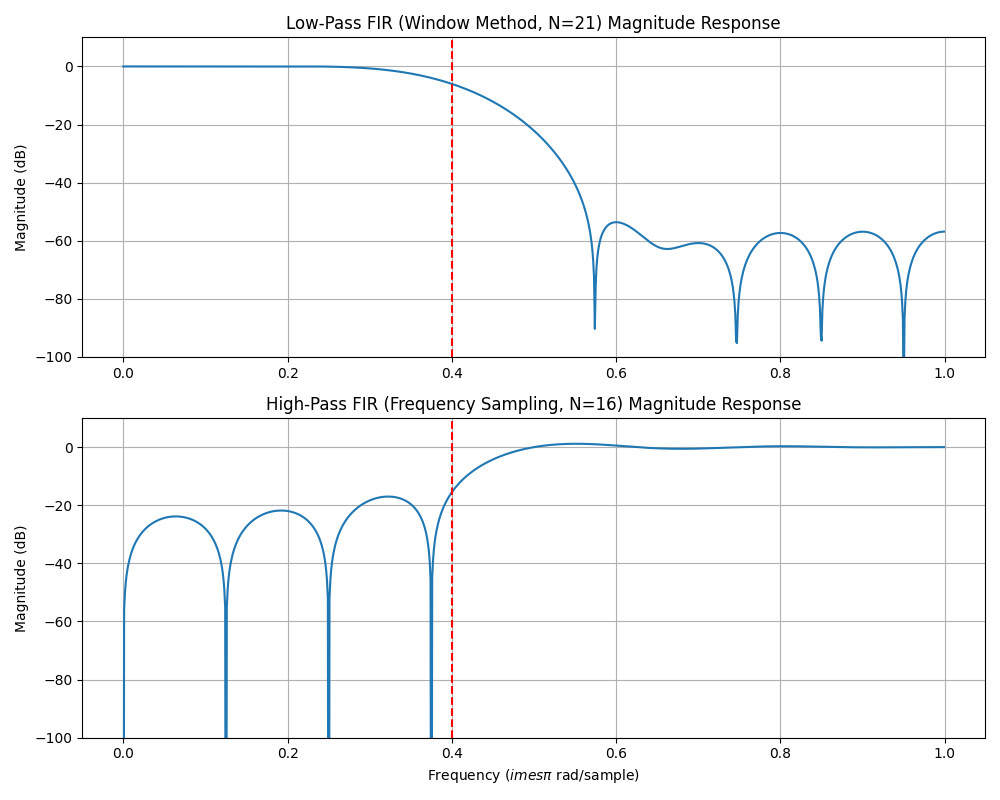
\includegraphics[width=0.8\textwidth]{plots/fir_comparison.png}
    \caption{Simulated Frequency Response Metrics for Disparate FIR Configurations}
\end{figure}

\subsection{Comparison Discussion}
\begin{itemize}
    \item \textbf{Window Configuration (LPF, Hamming N=21):} Provides incredibly smooth passband behavior inherently blocking ripple formation due to the gradual roll-off properties scaling internal limits. The stop band attenuation settles securely below $-50$ dB. The drawback is its wide transition boundary mapping natively to the $4\pi/N$ window lobe limitation.
    \item \textbf{Frequency Sampling Configuration (HPF, N=16):} Enables explicit manipulation bridging the transition, hitting frequency bins explicitly on specific magnitudes mapping tight discrete transition intervals spanning the $0.4\pi$. However, intermediate points generate intense Gibbs phenomenon anomalies resulting in severe oscillatory passband ripple and shallow relative stopband attenuation lacking any explicit magnitude clamping formulas compared to continuous window derivatives.
\end{itemize}

\end{document}
